\documentclass[a4paper,12pt]{scrartcl}
\usepackage[utf8]{inputenc}
\usepackage[T1]{fontenc}
\usepackage[ngerman]{babel}
\usepackage[pdftex]{graphicx}
\usepackage[linktoc=all]{hyperref}
\usepackage{subfig}
\usepackage{algorithmic}
\usepackage{algorithm} 
\usepackage{listings} 
\usepackage{color} 
\usepackage[right]{eurosym}
\usepackage{booktabs}
\usepackage[babel,german=quotes]{csquotes}
\renewcommand{\thefootnote}{[\arabic{footnote}]}
\renewcommand{\cite}{\footcite}

\definecolor{dkgreen}{rgb}{0,0.6,0}
\definecolor{gray}{rgb}{0.5,0.5,0.5}
\definecolor{mauve}{rgb}{0.58,0,0.82}

\title{Projektbericht 5. Semester}
\author{Name1 und Name2}
\date{\today}
\begin{document}
\linespread{1.5}
\maketitle 

\begin{abstract} 
\noindent
Im Rahmen des embeddedOptiBiohash Projektes im 5. Semester sahen wir uns neben der Hauptaufgabe mit einer Reihe an weiteren Fragestellungen konfrontriert, die teils gegeben wurden aber \"uberwiegend selbst gestellt waren.
So haben wir uns unter anderem mit folgenden Fragen besch\"aftig:
\newline\noindent
Welche Lizenstechnischen Freiheiten haben wir? z.B. um Quelltext aus anderen (freien) Bibliotheken zu nutzen
\newline\noindent
Gibt es Dokumentation zum Quelltext, bzw Minimalbeispiele um sich reinzufinden und mit der Plattform vertraut zu machen?
\newline\noindent	
Gibt es alternativen zur propriet\"aren IDE, die in zur Verf\"ugung gestellten Evaluierungsversion nur recht kleine Firmare flashen kann, die ohne technische Einschr\"ankungne Funktioniert und auf richtigen Betriebssystemen l\"auft?
\newline\noindent	
Wie verhalten sich die biometrischen Daten bei simulierten Alterungsprozessen?
\newline\noindent	
Im nachhinein Implementieren wir dann - die eigentliche Aufgabe- ein Konzept f\"ur eine m\"ogliche graphische Oberfl\"ache, die den Biohash auf dem Ger\"at nutzbar macht.
Die Dokumentation unterteilt sich gem\"a{\ss} der einzelnen Arbeitspakete in autarke Abschnitte, die auch losgel\"ost voneinander stehen k\"onnen.
\end{abstract}

\begin{figure}
  	\centering
    	
\includegraphics[scale=0.25]{img/fhlogo.jpg}
\end{figure}


\newpage
\tableofcontents
\newpage
\section{Organisation}

Die allgemeine Kommunikation war gut, die meist w\"ochentlichen Meetings zum feststellen des Fortschrittes und absprechen der n\"achsten schritte ebenso. Unterst\"utzend k\"onnte man dazu Projektverwaltungssoftware wie Trac oder Redmine einsetzen, bei der auch Arbeitspakete erstellt, gewissen Personen als Bearbeiter und anderen als Hypervisor zugewiesen werden k\"onnen. Damit kann man den Fortschritt auch gut verfolgen,wenn man sich mal nicht trifft und man selbst sieht auch auf einem Blick wo man steht.

Zudem hat man durch die Notizen zur den Arbeitspaketen auch gleiche eine Art Doku, wodurch sich der Aufwand daf\"ur minimieren w\"urde.
Eine Intensivere nutzung von SCM,  bzw erstmal ein zuverl\"assiges und Zeitgem\"a{\ss}es SCM w\"ar auch w\"unschenswert. In Projekten mit mehreren Entwicklern, die auch verteilt arbeiten sollte sowas heutzutage zum allgemeinen Arbeitsfluss geh\"oren. 
Die vorteile daf\"ur sind  gem\"a{\ss} der Device "commit early and often" man selbst und andere sehen sofort was als letztes ver\"andert wurde und in einem kurzen knackigen Kommentar f\"ur die Log auch ohne in die Source zu gucken. man kann das ganze auch ein Bugtrackingsystem koppeln (siehe trac/redmine) und kann Bugs fillen und zu den commits zuordnen. Es kann auch ein Buildserver angebunden werden, der je nach policy  z.b. commitgesteuert Testet (siehe TDD) oder einfach so versucht das Projekt zu bauen und bei einem Fehler wird sofort Alarm geschlagen um regressionen zu vermeiden.

Eine zus\"atzliche Verbesserung w\"are es die Quelltexte durch ein Dokutool (z.b Doxygen) zu jagen um damit eine dedizierte Dokumentation \"uber die Funktionen, quasi der API, zu haben. So kann man auch mal au{\ss}erhalb der Entwicklungsumgebung sich gedanken zum Programmablauf machen.
\newpage
\section{Implementierung}

Die Implementierung gestalltete sich \"uberwiegend in der main.c. Da diese mit am schlechtesten auskommentiert war, war eine Rekapitulaion des bereits vorhandenen Quellcodes sehr schwierig. Wir entschlossen uns daher die main.c schrittweise neu herzuleiten und die Verwendung der einzelnen Headerdateien zu verstehen. Die ersten GUIs die somit entstanden waren einfache Konstrukte aus Linien und Text. Im n\"achsten Schritt implementierten wir die ersten Buttons und die dazugeh\"origen Funktionen. Aufbauend darauf enstand ein simpler Taschenrechner f\"ur dessen Eingabe ein 3x4 Pinpad und jeweils ein Button f\"ur die jeweilige Grundrechenart. Wir kamen danach zu dem Punkt an dem wir uns ein Konzept f\"ur die eigentliche Nutzeroberfl\"ache \"uberlegen mussten. Dabei entschieden wir uns f\"ur die Men\"uf\"uhrung welche bereits in der orgninalen main.c implementiert war, da diese durch die Men\"uauswahl auf der rechten Displayseite eine intuitive Bedienung erm\"oglichte. Die Men\"upunkte erm\"oglichen dem Nutzer Zugriff auf die Enrollement-, Verifikations- u. Konfigurationsfunktionen zu nehmen. Nach der Initialisierung wird auf dem Display eine Willkommensanzeige dargestellt. (Abbildung \ref{welcScreen}) Beim Enrollement und der Verifikation werden jeweils 8 Buttons angezeigt welche f\"ur die Auswahl des aktuellen Nutzers zust\"adnig sind. Die Buttons wurden einem Frame in der Anordung 4x2 zugeordnet, damit mussten wir die Buttons nicht einzeln zeichnen lassen sondern konnten durch ein einmaliges zeichnen des Frames alle Buttons darstellen. (Abbildung \ref{Pic2}) Um den Quellcode weiterhin zu verk\"urzen nutzten wir den Frame mit den Buttons wie bereits erw\"ahnt sowohl f\"ur den Enrollementprozess sowie f\"ur die Verifikation. Das hei{\ss}t bei einem Klickevent wird die Abfrage gestellt welche Men\"upunkt aktiviert ist und erst danach erfolgt der Aufruf der Funktion. Diese Funktion ist bisweilen aber nur f\"ur User1 implementiert. Um die Tresholdeinstellung aus dem Konfigurationsmen\"u in die Verifikation mit einflie{\ss}en zu lassen haben wir die Funktion daf\"ur geringf\"ugig modifiziert. Wir haben einen zus\"atzlichen \"ubergabeparameter und eine Abfrage ob die Hammingdistanz den gesetzten Treshold \"uberschritten hat hinzugef\"ugt. Ausserdem erfolgt in der Funktion noch die Ausgabe ob die Verifikation erfolgreich war oder eben nicht.(Abbildung \ref{Pic3}) Das zweite Frame ist demzufolge f\"ur das Konfigurationsmen\"u geschaffen. Dort besteht die M\"oglichkeit den Treshold f\"ur eine g\"ultige bzw. ung\"ultige Verifikation auf die Werte 5, 10, 15 und 20 zu setzten (Abbildung \ref{TreshScreen}). Sollte hier keine weitere Einstellung des Nutzers erfolgen wird die Verifikation mit einem Treshold von 10 durchgef\"uhrt. \footnote{\label{foot:1} Quellcode: \ref{quellcode}}

 \begin{figure}
  \centering
  \subfloat[]{\label{welcScreen}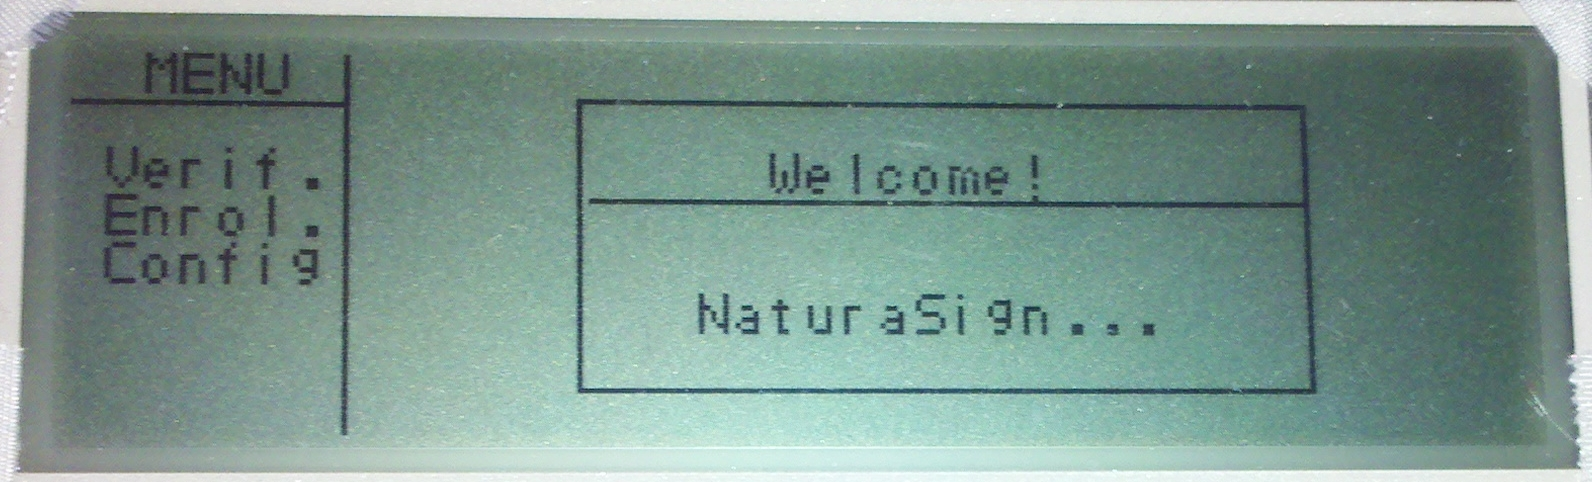
\includegraphics[width=0.5\textwidth]{img/welcScreen.jpg}}
  \subfloat[]{\label{TreshScreen}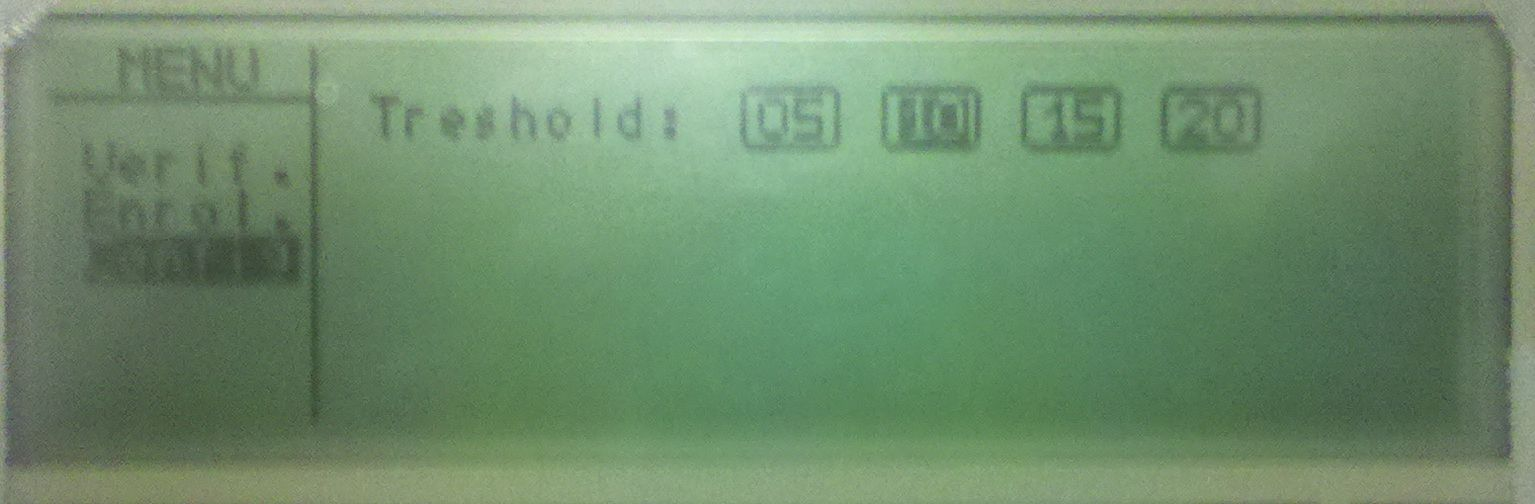
\includegraphics[width=0.46\textwidth]{img/TreshScreen.jpg}}
  \caption{Willkommensanzeige und Konfigurationsmen\"u}
  \label{Pic1}
\end{figure}

 \begin{figure}
  \centering
  \subfloat[]{\label{veriScreen}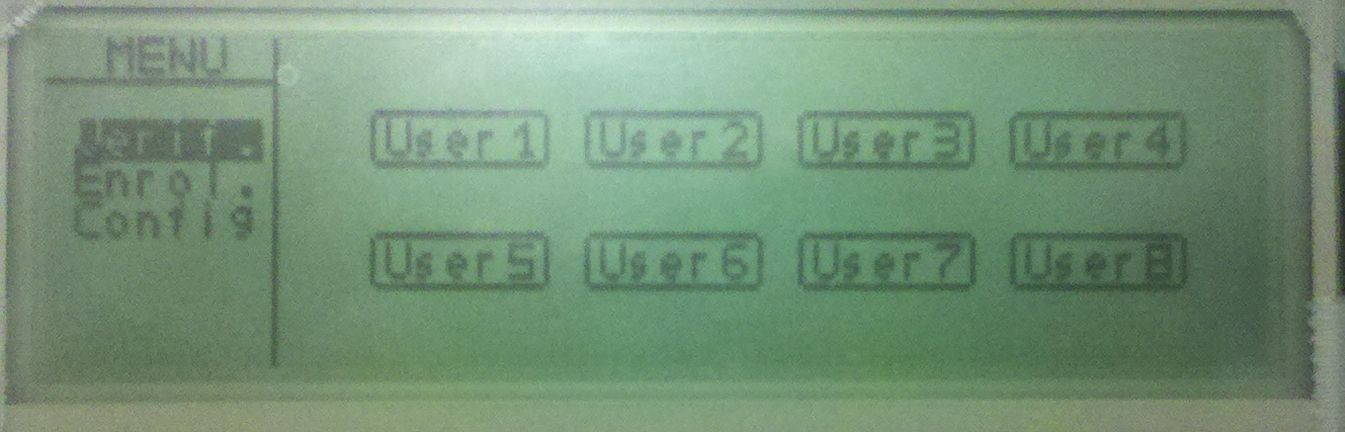
\includegraphics[width=0.5\textwidth]{img/veriScreen.jpg}}
  \subfloat[]{\label{enrolScreen}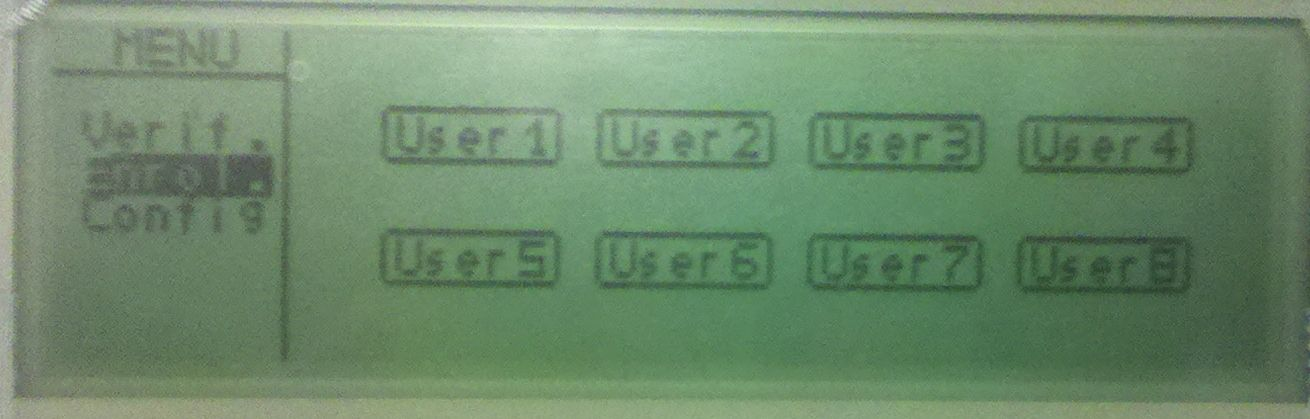
\includegraphics[width=0.50\textwidth]{img/enrolScreen.jpg}}
  \caption{Nutzerauswahl beim Enrollment und der Verifikation}
  \label{Pic2}
\end{figure}

 \begin{figure}
  \centering
  \subfloat[]{\label{failScreen}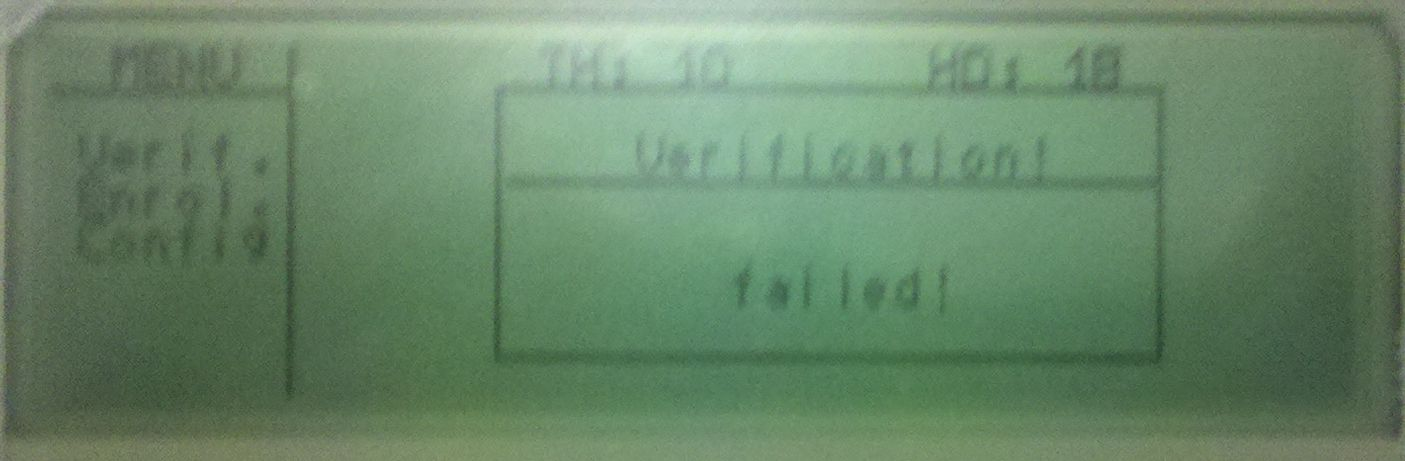
\includegraphics[width=0.48\textwidth]{img/failScreen.jpg}}
  \subfloat[]{\label{succesScreen}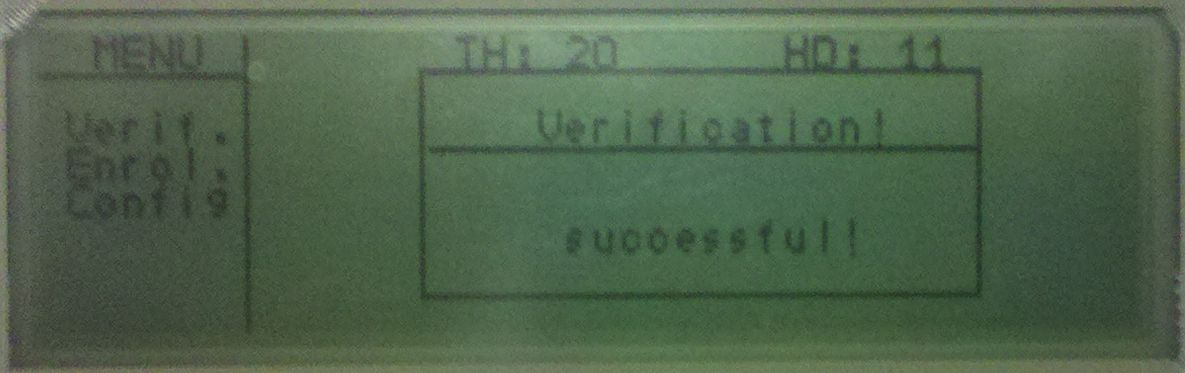
\includegraphics[width=0.50\textwidth]{img/succesScreen.jpg}}
  \caption{Ergebnisse der Verifikation}
  \label{Pic3}
\end{figure}

		
	\begin{figure}
  	\centering
  	\fbox{
    	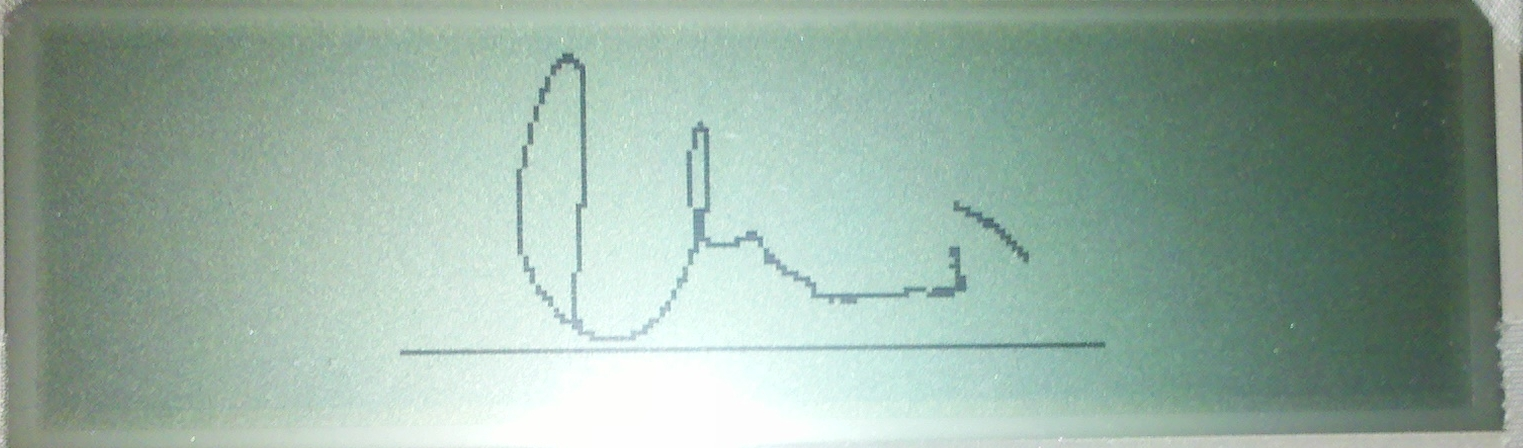
\includegraphics[scale=0.70]{img/graphScreen.jpg}
  	}
  	\caption{Unterschrift}
  	\label{graphScreen}
	\end{figure}
	
		
	
\newpage
\section{Alterungstest in Matlab}

F\"ur die Vergleiche der einzelnen Datens\"atze war es notwendig den vorhandenen Quellcode zu modifizieren. Anfangs stand also prim\"ar das Verst\"andnis f\"ur den Hashalgorithmus als solchen sowie dessen Implementierung in Matlab im Vordergrund. Dies nahm einige Zeit in Anspruch, da die Umsetzung des Algorithmus zwar mathematisch kompakt aber dadurch schwer verst\"andlich, implementiert worden ist. Als der Quellcode ausreichend modifiziert war fiel uns nach der ersten Versuchsreihe auf, dass die Werte unrealistisch hoch bis hin zu unm\"oglich waren. Indiz daf\"ur war, dass die Kollisionsrate und die Reproduktionsrate jedesmal bei 0 lag. Dies h\"atte eine Verifizierung unm\"oglich gemacht. Die Ursache daf\"ur war letztendlich, dass f\"ur die Simulation ein Toleranzvektor mit dem Wert 0 verwendet wurde. Um also realistischere Werte zu erzielen setzten wir diesen auf 1 mit dem Ergebniss, dass sich die Aussagekraft der Werte deutlich besserte. Nach der ersten Versuchsreihe fiel uns auf, dass die Ergebnis unrealistisch bis hin zu unm\"oglich waren. Indiz daf\"ur war dass die CR und die RR jedesmal bei 0 lag. Was eine Verifizierung unm\"oglich gemacht h\"atte. Ebenfalls war der Treshold zu hoch. Uns fiel uns dann auf, dass die Ursache hierf\"ur der Toleranzvektor war. Dieser war in der bisherigen Umsetzung immer auf 0. F\"ur das weitere Testverfahren nutzen wir dann einen Toleranzvektor von 1. Anschlie{\ss}end hatten die Ergebnisse auch eine wesentlich bessere Aussagekraft. 
Die besten Ergebnisse lieferten die Daten welche zeitnah aufgenommen und auch verifiziert wurden. Die Durchschnittswerte betrugen dabei:
\newline\newline
\centerline{$EER:$ 0,027950  $Treshold:$ 13,0561  $RR:$ 0,064906}
\newline\newline\noindent
Diese sind deutlich geringer als der Vergleich der Samples welche einen zeitlichen Abstand von 1-2 Monaten haben. Hierbei liegen die Durchschnittswerte bei: 
\newline\newline
\centerline{$EER:$ 0,104641  $Treshold:$ 19,8423  $RR:$ 0,010566}
\newline\newline\noindent
\"Ahnliche Werte wurden auch beim Vergleich j\"ungerer Referenzdaten mit \"alteren Verifikationsdaten (Tabelle \ref{tab:reverse}), \"alterer Referenzdaten mit neueren Referenzdaten (Tabelle \ref{tab:referenz}) und  \"alterer Verifikationsdaten mit neueren Verifikationsdaten (Tabelle \ref{tab:verifikation}). Zwischen der Aufnahme dereinzelnen Datens\"atze lag jeweils ein Zeitraum von einem Monat. Basierend auf diesen Daten haben wir dann bei der Implementation auf dem Ger\"at einen maximalen Treshold von 20 gew\"ahlt.
\newpage
% Table generated by Excel2LaTeX from sheet 'Reverse'
\begin{table}[htbp]
  \centering
  \caption{j\"ungere Referenzdaten vs \"altere Verifikationsdaten}
    \begin{tabular}{rrrrrr}
    \toprule
    \textbf{R2 vs. V1} & \multicolumn{1}{c}{EER} & \multicolumn{1}{c}{Thr.:} & \multicolumn{1}{c}{RR} & \multicolumn{1}{c}{CR} & \multicolumn{1}{c}{CRR} \\
    \midrule
    77993 & \multicolumn{1}{c}{0,183870} & \multicolumn{1}{c}{19,5686} & \multicolumn{1}{c}{0,007547} & \multicolumn{1}{c}{0} & \multicolumn{1}{c}{0,496230} \\
    pin   & \multicolumn{1}{c}{0,135180} & \multicolumn{1}{c}{18,2946} & \multicolumn{1}{c}{0,007547} & \multicolumn{1}{c}{0} & \multicolumn{1}{c}{0,496230} \\
    pseudonym & \multicolumn{1}{c}{0,109580} & \multicolumn{1}{c}{23,4906} & \multicolumn{1}{c}{0,003774} & \multicolumn{1}{c}{0} & \multicolumn{1}{c}{0,498110} \\
    symbol & \multicolumn{1}{c}{0,144660} & \multicolumn{1}{c}{25,6645} & \multicolumn{1}{c}{0,003774} & \multicolumn{1}{c}{0} & \multicolumn{1}{c}{0,498110} \\
    woher & \multicolumn{1}{c}{0,093405} & \multicolumn{1}{c}{24,7493} & \multicolumn{1}{c}{0,011321} & \multicolumn{1}{c}{0} & \multicolumn{1}{c}{0,494340} \\
          &       &       &       &       &  \\
          &       &       &       &       &  \\
    \textbf{R3 vs. V1} & \multicolumn{1}{c}{EER} & \multicolumn{1}{c}{Thr.:} & \multicolumn{1}{c}{RR} & \multicolumn{1}{c}{CR} & \multicolumn{1}{c}{CRR} \\
    77993 & \multicolumn{1}{c}{0,206380} & \multicolumn{1}{c}{20,0517} & \multicolumn{1}{c}{0,000000} & \multicolumn{1}{c}{0} & \multicolumn{1}{c}{0,500000} \\
    pin   & \multicolumn{1}{c}{0,193000} & \multicolumn{1}{c}{20,9760} & \multicolumn{1}{c}{0,000000} & \multicolumn{1}{c}{0} & \multicolumn{1}{c}{0,500000} \\
    pseudonym & \multicolumn{1}{c}{0,137170} & \multicolumn{1}{c}{25,3649} & \multicolumn{1}{c}{0,003774} & \multicolumn{1}{c}{0} & \multicolumn{1}{c}{0,498110} \\
    symbol & \multicolumn{1}{c}{0,156560} & \multicolumn{1}{c}{23,9185} & \multicolumn{1}{c}{0,007547} & \multicolumn{1}{c}{0} & \multicolumn{1}{c}{0,496230} \\
    woher & \multicolumn{1}{c}{0,098103} & \multicolumn{1}{c}{23,6676} & \multicolumn{1}{c}{0,015094} & \multicolumn{1}{c}{0} & \multicolumn{1}{c}{0,492450} \\
          &       &       &       &       &  \\
          &       &       &       &       &  \\
    \textbf{R3 vs. V2} & \multicolumn{1}{c}{EER} & \multicolumn{1}{c}{Thr.:} & \multicolumn{1}{c}{RR} & \multicolumn{1}{c}{CR} & \multicolumn{1}{c}{CRR} \\
    77993 & \multicolumn{1}{c}{0,121180} & \multicolumn{1}{c}{15,8864} & \multicolumn{1}{c}{0,007547} & \multicolumn{1}{c}{0} & \multicolumn{1}{c}{0,496230} \\
    pin   & \multicolumn{1}{c}{0,116660} & \multicolumn{1}{c}{16,6171} & \multicolumn{1}{c}{0,011321} & \multicolumn{1}{c}{0} & \multicolumn{1}{c}{0,494340} \\
    pseudonym & \multicolumn{1}{c}{0,103180} & \multicolumn{1}{c}{23,3284} & \multicolumn{1}{c}{0,022642} & \multicolumn{1}{c}{0} & \multicolumn{1}{c}{0,488680} \\
    symbol & \multicolumn{1}{c}{0,053443} & \multicolumn{1}{c}{16,4594} & \multicolumn{1}{c}{0,018868} & \multicolumn{1}{c}{0} & \multicolumn{1}{c}{0,490570} \\
    woher & \multicolumn{1}{c}{0,078964} & \multicolumn{1}{c}{22,3582} & \multicolumn{1}{c}{0,022642} & \multicolumn{1}{c}{0} & \multicolumn{1}{c}{0,488680} \\
          &       &       &       &       &  \\
          &       &       &       &       &  \\
    \bottomrule
    \end{tabular}%
  \label{tab:reverse}%
\end{table}%

% Table generated by Excel2LaTeX from sheet 'Rx vs Ry'
\begin{table}[htbp]
  \centering
  \caption{\"altere Referenzdaten vs neuere Referenzdaten}
    \begin{tabular}{rrrrrr}
    \toprule
    \textbf{R1 vs. R2} & \multicolumn{1}{c}{EER} & \multicolumn{1}{c}{Thr.:} & \multicolumn{1}{c}{RR} & \multicolumn{1}{c}{CR} & \multicolumn{1}{c}{CRR} \\
    \midrule
    77993 & \multicolumn{1}{c}{0,171200} & \multicolumn{1}{c}{17,3263} & \multicolumn{1}{c}{0,003774} & \multicolumn{1}{c}{0} & \multicolumn{1}{c}{0,498110} \\
    pin   & \multicolumn{1}{c}{0,128400} & \multicolumn{1}{c}{17,2437} & \multicolumn{1}{c}{0,011321} & \multicolumn{1}{c}{0} & \multicolumn{1}{c}{0,494340} \\
    pseudonym & \multicolumn{1}{c}{0,093423} & \multicolumn{1}{c}{20,8107} & \multicolumn{1}{c}{0,007547} & \multicolumn{1}{c}{0} & \multicolumn{1}{c}{0,496230} \\
    symbol & \multicolumn{1}{c}{0,074450} & \multicolumn{1}{c}{19,2118} & \multicolumn{1}{c}{0,003774} & \multicolumn{1}{c}{0} & \multicolumn{1}{c}{0,498110} \\
    woher & \multicolumn{1}{c}{0,094381} & \multicolumn{1}{c}{20,4945} & \multicolumn{1}{c}{0,000000} & \multicolumn{1}{c}{0} & \multicolumn{1}{c}{0,500000} \\
          &       &       &       &       &  \\
          &       &       &       &       &  \\
    \textbf{R1 vs. R3} & \multicolumn{1}{c}{EER} & \multicolumn{1}{c}{Thr.:} & \multicolumn{1}{c}{RR} & \multicolumn{1}{c}{CR} & \multicolumn{1}{c}{CRR} \\
    77993 & \multicolumn{1}{c}{0,227050} & \multicolumn{1}{c}{18,9436} & \multicolumn{1}{c}{0,003774} & \multicolumn{1}{c}{0} & \multicolumn{1}{c}{0,498110} \\
    pin   & \multicolumn{1}{c}{0,173500} & \multicolumn{1}{c}{18,8044} & \multicolumn{1}{c}{0,007547} & \multicolumn{1}{c}{0} & \multicolumn{1}{c}{0,496230} \\
    pseudonym & \multicolumn{1}{c}{0,115290} & \multicolumn{1}{c}{21,9081} & \multicolumn{1}{c}{0,011321} & \multicolumn{1}{c}{0} & \multicolumn{1}{c}{0,494340} \\
    symbol & \multicolumn{1}{c}{0,104090} & \multicolumn{1}{c}{20,5692} & \multicolumn{1}{c}{0,018868} & \multicolumn{1}{c}{0} & \multicolumn{1}{c}{0,490570} \\
    woher & \multicolumn{1}{c}{0,120010} & \multicolumn{1}{c}{22,0654} & \multicolumn{1}{c}{0,015094} & \multicolumn{1}{c}{0} & \multicolumn{1}{c}{0,492450} \\
          &       &       &       &       &  \\
          &       &       &       &       &  \\
    \textbf{R2 vs. R3} & \multicolumn{1}{c}{EER} & \multicolumn{1}{c}{Thr.:} & \multicolumn{1}{c}{RR} & \multicolumn{1}{c}{CR} & \multicolumn{1}{c}{CRR} \\
    77993 & \multicolumn{1}{c}{0,144320} & \multicolumn{1}{c}{16,3755} & \multicolumn{1}{c}{0,011321} & \multicolumn{1}{c}{0} & \multicolumn{1}{c}{0,494380} \\
    pin   & \multicolumn{1}{c}{0,113010} & \multicolumn{1}{c}{16,4593} & \multicolumn{1}{c}{0,003774} & \multicolumn{1}{c}{0} & \multicolumn{1}{c}{0,498110} \\
    pseudonym & \multicolumn{1}{c}{0,077918} & \multicolumn{1}{c}{21,1759} & \multicolumn{1}{c}{0,007547} & \multicolumn{1}{c}{0} & \multicolumn{1}{c}{0,496230} \\
    symbol & \multicolumn{1}{c}{0,088011} & \multicolumn{1}{c}{20,7354} & \multicolumn{1}{c}{0,030189} & \multicolumn{1}{c}{0} & \multicolumn{1}{c}{0,484910} \\
    woher & \multicolumn{1}{c}{0,060803} & \multicolumn{1}{c}{22,1775} & \multicolumn{1}{c}{0,011321} & \multicolumn{1}{c}{0} & \multicolumn{1}{c}{0,494340} \\
          &       &       &       &       &  \\
          &       &       &       &       &  \\
    \bottomrule
    \end{tabular}%
  \label{tab:referenz}%
\end{table}%

% Table generated by Excel2LaTeX from sheet 'Vx vs Vy'
\begin{table}[htbp]
  \centering
  \caption{\"altere Verifikationsdaten vs neuere Verifikationsdaten}
    \begin{tabular}{rrrrrr}
    \toprule
    \textbf{V1 vs. V2} & \multicolumn{1}{c}{EER} & \multicolumn{1}{c}{Thr.:} & \multicolumn{1}{c}{RR} & \multicolumn{1}{c}{CR} & \multicolumn{1}{c}{CRR} \\
    \midrule
    77993 & \multicolumn{1}{c}{0,147440} & \multicolumn{1}{c}{21,6426} & \multicolumn{1}{c}{0,000000} & \multicolumn{1}{c}{0} & \multicolumn{1}{c}{0,500000} \\
    pin   & \multicolumn{1}{c}{0,132110} & \multicolumn{1}{c}{19,9980} & \multicolumn{1}{c}{0,007547} & \multicolumn{1}{c}{0} & \multicolumn{1}{c}{0,496230} \\
    pseudonym & \multicolumn{1}{c}{0,089150} & \multicolumn{1}{c}{25,2292} & \multicolumn{1}{c}{0,000000} & \multicolumn{1}{c}{0} & \multicolumn{1}{c}{0,500000} \\
    symbol & \multicolumn{1}{c}{0,132170} & \multicolumn{1}{c}{25,3248} & \multicolumn{1}{c}{0,026415} & \multicolumn{1}{c}{0} & \multicolumn{1}{c}{0,486790} \\
    woher & \multicolumn{1}{c}{0,072075} & \multicolumn{1}{c}{24,2250} & \multicolumn{1}{c}{0,000000} & \multicolumn{1}{c}{0} & \multicolumn{1}{c}{0,500000} \\
          &       &       &       &       &  \\
          &       &       &       &       &  \\
    \textbf{V1 vs. V3} & \multicolumn{1}{c}{EER} & \multicolumn{1}{c}{Thr.:} & \multicolumn{1}{c}{RR} & \multicolumn{1}{c}{CR} & \multicolumn{1}{c}{CRR} \\
    77993 & \multicolumn{1}{c}{0,161760} & \multicolumn{1}{c}{21,7612} & \multicolumn{1}{c}{0,000000} & \multicolumn{1}{c}{0} & \multicolumn{1}{c}{0,500000} \\
    pin   & \multicolumn{1}{c}{0,161990} & \multicolumn{1}{c}{20,5092} & \multicolumn{1}{c}{0,003774} & \multicolumn{1}{c}{0} & \multicolumn{1}{c}{0,498110} \\
    pseudonym & \multicolumn{1}{c}{0,125430} & \multicolumn{1}{c}{27,2934} & \multicolumn{1}{c}{0,003774} & \multicolumn{1}{c}{0} & \multicolumn{1}{c}{0,498110} \\
    symbol & \multicolumn{1}{c}{0,140030} & \multicolumn{1}{c}{25,6114} & \multicolumn{1}{c}{0,015094} & \multicolumn{1}{c}{0} & \multicolumn{1}{c}{0,492450} \\
    woher & \multicolumn{1}{c}{0,087514} & \multicolumn{1}{c}{25,1348} & \multicolumn{1}{c}{0,007547} & \multicolumn{1}{c}{0} & \multicolumn{1}{c}{0,496230} \\
          &       &       &       &       &  \\
          &       &       &       &       &  \\
    \textbf{V2 vs. V3} & \multicolumn{1}{c}{EER} & \multicolumn{1}{c}{Thr.:} & \multicolumn{1}{c}{RR} & \multicolumn{1}{c}{CR} & \multicolumn{1}{c}{CRR} \\
    77993 & \multicolumn{1}{c}{0,142370} & \multicolumn{1}{c}{18,8079} & \multicolumn{1}{c}{0,011321} & \multicolumn{1}{c}{0} & \multicolumn{1}{c}{0,494340} \\
    pin   & \multicolumn{1}{c}{0,105540} & \multicolumn{1}{c}{19,5032} & \multicolumn{1}{c}{0,011321} & \multicolumn{1}{c}{0} & \multicolumn{1}{c}{0,494340} \\
    pseudonym & \multicolumn{1}{c}{0,077908} & \multicolumn{1}{c}{25,6772} & \multicolumn{1}{c}{0,007547} & \multicolumn{1}{c}{0} & \multicolumn{1}{c}{0,496230} \\
    symbol & \multicolumn{1}{c}{0,049057} & \multicolumn{1}{c}{21,6198} & \multicolumn{1}{c}{0,015094} & \multicolumn{1}{c}{0} & \multicolumn{1}{c}{0,492450} \\
    woher & \multicolumn{1}{c}{0,075088} & \multicolumn{1}{c}{25,0508} & \multicolumn{1}{c}{0,003774} & \multicolumn{1}{c}{0} & \multicolumn{1}{c}{0,498110} \\
          &       &       &       &       &  \\
          &       &       &       &       &  \\
    \bottomrule
    \end{tabular}%
  \label{tab:verifikation}%
\end{table}%


\newpage
\section{Quellcode}
\label{quellcode}

\subsection{main.c}
\label{main}
\lstinputlisting [language =C++,  
									basicstyle=\footnotesize,           
  								numbers=left,                   
  								numberstyle=\tiny\color{gray},  
  								stepnumber=2,
  								numbersep=5pt,                  
    							backgroundcolor=\color{white},     
 									showspaces=false,               
  								showstringspaces=false,         
    							showtabs=false,                 
    							frame=single,                  
    							rulecolor=\color{black},       
  								tabsize=2,                     
  								captionpos=b,                  
  								breaklines=true,                
  								breakatwhitespace=false,        
  								title=\lstname,                   
  								keywordstyle=\color{blue},          
 									commentstyle=\color{dkgreen},       
  								stringstyle=\color{mauve}]{src/main.cpp }
  								
\subsection{authentication.c}
\label{authenticatio}
\lstinputlisting [language =C++,  
									basicstyle=\footnotesize,           
  								numbers=left,                   
  								numberstyle=\tiny\color{gray},  
  								stepnumber=2,
  								numbersep=5pt,                  
    							backgroundcolor=\color{white},     
 									showspaces=false,               
  								showstringspaces=false,         
    							showtabs=false,                 
    							frame=single,                  
    							rulecolor=\color{black},       
  								tabsize=2,                     
  								captionpos=b,                  
  								breaklines=true,                
  								breakatwhitespace=false,        
  								title=\lstname,                   
  								keywordstyle=\color{blue},          
 									commentstyle=\color{dkgreen},       
  								stringstyle=\color{mauve}]{src/veri.cpp }

%\input{}
%.......
%.......
%:......
%\input{}
\newpage
%.......
%\input{}
\end{document}

